\documentclass[12pt]{article}

\usepackage{graphicx}
\usepackage{geometry}
\usepackage{multicol}

\geometry{
    top=20mm,
    bottom=20mm,
    right=20mm,
    left=20mm
}

\title{WMATH1010 Problem Set 3}
\author{Ben Crause || Aayush Bajaj}


\begin{document}
\maketitle{}

\section*{Question 1}
\[
    2\ln(x+2) + \frac{3}{2} \ln(x^2 + 6x + 13) + \frac{1}{2} \arctan(\frac{x}{2} + \frac{3}{2}) + C
\]

\section*{Question 2}

\subsection*{a)}
\[V = \frac{9 \pi}{10} u^3\]

\begin{center}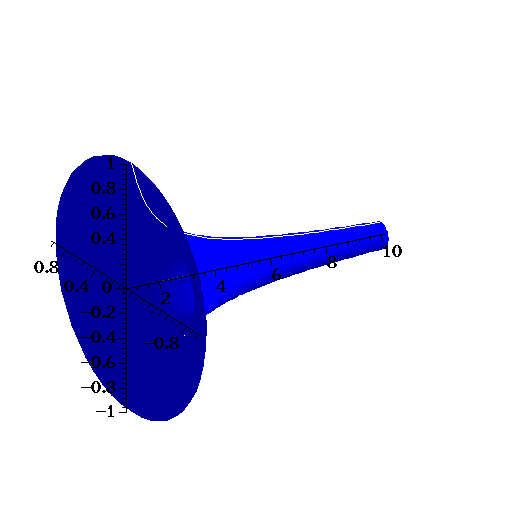
\includegraphics[width=0.5\textwidth, trim={2cm 1cm 2cm 3cm},clip]{plots/q2a.png}\end{center}
    %  trim={<left> <lower> <right> <upper>}

\newpage
\subsection*{b)}
\[
    V = \frac{\pi^2}{2}u^3    
\]
\begin{center}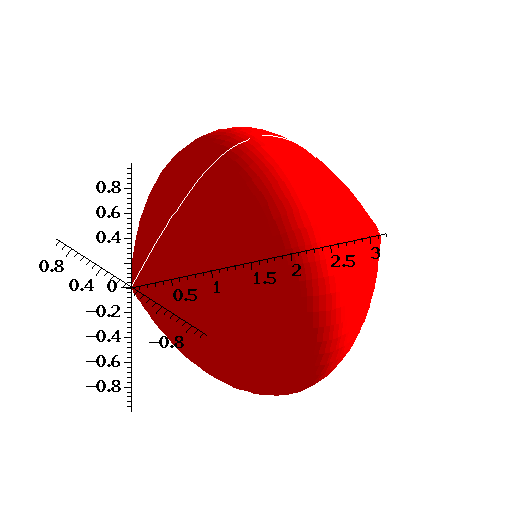
\includegraphics[width=0.5\textwidth, trim={2cm 1cm 2cm 3cm},clip]{plots/q2b.png}\end{center}

\subsection*{c)}
\[
    V = \frac{7533 \pi}{5} u^3
\]
\begin{center}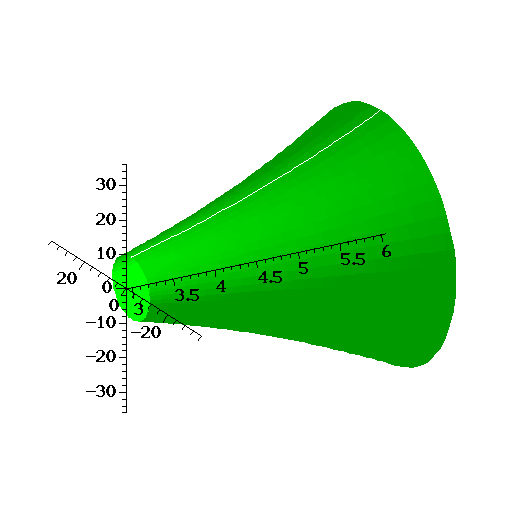
\includegraphics[width=0.5\textwidth, trim={2cm 1cm 2cm 3cm},clip]{plots/q2c.png}\end{center}

\section*{Question 3}

\section*{Question 4}

\end{document}
